% Styling and set-up
\documentclass{article}


\usepackage{NotesStyle}
\graphicspath{./figs/}

% Cover info

\title{Phys 514 \\
	\large Relativity}

\author{April Sada Solomon}
\date{Winter 2021}


% Document
\begin{document}

	\clearpage
	% Displays title info
	\maketitle
	
	\vspace{2cm}
	
	% Course description, displayed on cover page
	\renewcommand{\abstractname}{Course Description}
	\begin{abstract}
		 Notes taken directly from the lectures given by Dr. Maloney (not proof read by him). Special Relativity, Manifolds, Spacetime Curvature, Gravitation, Schwarzchild Solution, Black Holes, Perturbations, Radiation, Introduction to Cosmology, Introduction to QFT in Spacetime. 
	\end{abstract}
	
	\newpage
	
	\tableofcontents
	
	\newpage
	
	% Start page count after the TOC
	\setcounter{page}{1}
	\cfoot{\thepage}
	
	% Notes body
	\section{A Brief Review of Special Relativity}
	\subsection{Introduction}
 		General Relativity is the modern theory of classical gravity. What do we mean by "classical"? Simply, it is a nomenclature to distinguish from Quantum Mechanics, so those effects are ignored. The basic idea from Newtonian Mechanics is that gravity is a force, and as we know, most forces are described by fields.
 		
 		The simplest example of a field that describes a force is the Newtonian gravitational potential $\Phi (\vec{r})$:
 		\begin{equation}
 			\label{eq:NetwonGravitation}
 			\frac{d}{dt}\frac{\partial \Lgr}{\partial \dot{x}} = \frac{\partial \Lgr}{\partial x} \implies \vec{F} (\vec{v}) = - \frac{\partial}{\partial \vec{r}} \Phi (\vec{r}) 
 		\end{equation}
 		\noindent
 		If we are studying electromagnetism, we would study the electromagnetic fields $\vec{E}$ and $\vec{B}$. Let us list the Maxwell Equations, that we will review again later on:
 			\begin{align}
 				\label{eq:Maxwell}
 				\grad \cdot \vec{E} &= \frac{\rho}{\varepsilon_0} \\
 				\grad \cdot \vec{B} &= 0 \\
 				\grad \times \vec{E} &= -\frac{\partial \vec{B}}{\partial t} \\
 				\grad \times \vec{B} &= \mu_0 \left( \vec{J} + \varepsilon_0 \frac{\partial \vec{E}}{\partial t} \right)
 			\end{align}
 		A classical field theory like the theory of Newtonian gravity or the theory of Electromagnetism has two parts that describe it:
 		\begin{enumerate}
 			\item \textbf{Field equation}
 				\subitem A field equation is an equation of motion that describes exactly how a certain field is determined by some set of sources. In other words, it is usually a second order differential equation that has to be solved to determine the field from some collection of sources. 
 			\begin{exmp}
 				Newtonian gravity field equation
 				$$ \nabla^2 \Phi = 4\pi G \rho$$
 				where $\rho$ is the mass density. We solve this Laplace's equation to determine the field. If $\rho$ is a $\grad(\vec{r})$ function such that it describes a point mass, which implies that
 				$\Phi \propto \nicefrac{1}{\vec{r}}$.
 			\end{exmp}
	 		\begin{exmp}
	 			Electromagnetic field equations. See the \hyperref[eq:Maxwell]{Maxwell's Equation's} above. In equation (1.2), we have that $\rho$ represents the charge density to determine the field in terms of the forces from some collection of charge sources.
	 		\end{exmp}
 		\pagebreak
 			\item \textbf{Force law}
 			\subitem The force law is an equation that determines how an object moves in the presence of a field. So we start by describing a collection of sources and how they describe some force field, and then we use the force law to determine how bodies in motion are affected by the force field using the force law.
 			\begin{exmp}
 				Newtonian force law
 				$$ \vec{F}(t, \vec{x}, \dot{\vec{x}}) = \frac{m}{2}\frac{d}{dt} \frac{\partial}{\partial \vec{v}}\vec{v}^2 = m \dot{\vec{v}} =- m \vec{\grad} \Phi(t,\vec{x}) $$
 				where $\dot{\vec{v}} = \nicefrac{d^2 \vec{x}}{dt^2} = \ddot{\vec{x}}$. This force law describes how some gravitational potential affects the motion of bodies in the presence of the field described by the potential.
 			\end{exmp}
 			\begin{exmp}
 				Lorentzian force law
 				$$ \vec{F} \left(t, \vec{x}, \dot{\vec{x}}\right)=q (\vec{E} + \vec{v} \times \vec{B} )$$
 				where $\vec{v} = \nicefrac{d\vec{x}}{dt} = \dot{\vec{x}}$.
 			\end{exmp}
 			The important thing here is that fields are just functions of points in spacetime. For example, the gravitational potential $\Phi (t, \vec{x})$ yields a number that depends on where you are in space time, and the electric field $\vec{E} (t, \vec{x})$ is also a vector that depends on where you are in space and time. We should think of force laws as equations that describe how the motion of objects deviate from being "straight lines". 
 		\end{enumerate}
 		To emphasize, let us assume that an object in inertial motion on the $+\hat{x}$ axis, neglecting field interactions with the object. Evidently so, it's acceleration is zero, yielding the differential equation $\ddot{x} = 0$. The solution to this second order differential equation yields motion in a straight line. So the force law considering a field with an object experiencing this motion will be able to distort the object's motion such that it is not a straight line anymore. For instance, a gravitational field will bend the straight line into a curve as it generates acceleration in the $-\hat{y}$ axis, leading to parabolic motion on the $\hat{x}\hat{y}-$plane.
 		
 		\begin{defn}
 			\textbf{General Relativity} is a complete reinterpretation of gravitation such that it is not a field using a potential $\Phi (t, \vec{x})$, but instead it is a feature of spacetime itself. In particular, we replace the gravitational potential with a \textit{metric tensor} that describes this feature, particularly, the geometrical curvature of spacetime.
 		\end{defn} 
 		We will be learning pseudo-Riemann topological spaces by employing Einstein's field equation, which determines how spacetime curvature is determined in the presence of matter or energy. In Newtonian gravitation, the source term was a mass (or energy density in Special Relativity where $E = mc^2$). Recall however that mass has no independent meaning in terms of relativity as energy and momentum both depend on the reference frame where they are measured. The "source" of the curvature in general relativity is a term in the Einstein field equations that describes a generalized mass-energy distribution in spacetime of the sources present.
 		
 		The force law is also replaced by the geodesic equation, which tells us how objects move through some curved spacetime. Particularly, the geometric interpretation of the geodesic is quite simple; it is the statement that \textit{object will move on \textbf{geodesics}, which are the shortest paths between two points on a surface.} In a flat surface, this is a straight line, but in curved surfaces, this trajectory will not be a straight line, like two points on the surface of a sphere.
 		
 		\begin{figure}[h]
 			\begin{subfigure}{0.46\textwidth}
 				\center
 				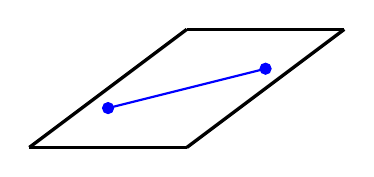
\begin{tikzpicture}
 					\draw [very thick] (0,0) -- (2,1.5);
 					\draw [very thick] (2,0) -- (4,1.5);
 					\draw [very thick] (0,0) -- (2,0);
 					\draw [very thick] (2,1.5) -- (4,1.5);
 					
 					\draw [thick, blue] (1, 0.5) -- (3, 1);
 					
 					\filldraw [blue] (1,0.5) circle (2pt)
 					(3,1) circle (2pt);
 				\end{tikzpicture}
 			\caption{Geodesic over a flat surface}
 			\end{subfigure}
 			\begin{subfigure}{0.46\textwidth}
 				\center
 				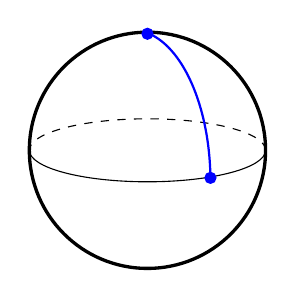
\begin{tikzpicture}
 					\draw [very thick] (0,0) circle (1.5cm);
 					\draw [dashed] (1.5,0) arc (0:180:1.5 and 0.4);
 					\draw (1.5,0) arc (0:180:1.5 and -0.4);
 					
 					\draw [thick, blue] (0.8, -0.35) arc (1.5:80:1 and 1.93);
 					
 					\filldraw [blue] (0.8,-0.35) circle (2pt)
 					(0,1.48) circle (2pt);
 				\end{tikzpicture}
 				\caption{Geodesic over a flat surface}
 			\end{subfigure}
 		\end{figure}
\end{document}